% Appendix A
\chapter{Appendix} % Main appendix title
\label{AppendixA} % For referencing this appendix elsewhere, use \ref{AppendixA}

\section{Project Structure}

\begin{figure}[htbp]
    \centering
    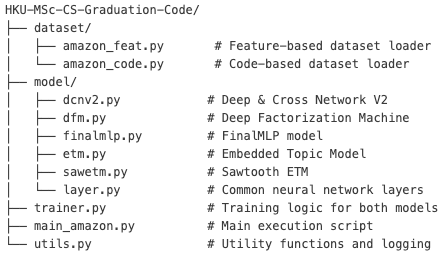
\includegraphics[width=0.5\textwidth]{Figures/proj_structure.png}
    \caption{Project Structure}
    \label{fig:proj_structure}
\end{figure}

\section{Key Components Analysis}

\subsection{Dataset Modules}

\subsubsection{AmazonDataset\_Feat (amazon\_feat.py)}

\begin{lstlisting}[language=Python, caption=Amazon Dataset Implementation]
class AmazonDataset_Feat(torch.utils.data.Dataset):
    def __init__(self, data, field_dims):
        self.items = data[['user_id','item_id']].values
        self.targets = data['label'].values
        self.field_dims = field_dims
\end{lstlisting}

\textbf{Purpose}: Handles basic user-item interaction data with binary labels for CTR prediction.

\subsubsection{ItemDataset\_Feat (amazon\_feat.py)}

\begin{lstlisting}[language=Python, caption=Item Dataset Implementation]
class ItemDataset_Feat(torch.utils.data.Dataset):
    def __init__(self, feat):
        self.embeddings = torch.FloatTensor(feat['embedding'])
        self.bow_data = torch.FloatTensor(feat['bow'].todense())
        self.vocab_embeddings = torch.FloatTensor(feat['vocab_emb'])
\end{lstlisting}

\textbf{Purpose}: Manages item features including:
\begin{itemize}
    \item Pre-trained embeddings (BERT-based)
    \item Bag-of-words representations for topic modeling
    \item Vocabulary embeddings
\end{itemize}

\subsection{Topic Models}

\subsubsection{ETM (Embedded Topic Model) (etm.py)}

\begin{lstlisting}[language=Python, caption=ETM Model Architecture]
class ETM(nn.Module):
    def __init__(self, args, device, word_embeddings):
        self.rho = nn.Parameter(word_embeddings)  # Word embeddings
        self.alpha = nn.Parameter(torch.empty(self.num_topics, self.embed_size))  # Topic embeddings
        self.h_encoder = ResBlock(self.vocab_size, self.num_hiddens, 'relu')
        self.q_theta = nn.Linear(self.num_hiddens, 2 * self.num_topics)
\end{lstlisting}

\textbf{Key Innovation}: Combines word embeddings with topic modeling:

\begin{lstlisting}[language=Python, caption=Topic-Word Matrix Derivation]
def get_phi(self):
    """Derives topic-word matrix by computing inner product"""
    dist = torch.mm(self.rho, self.alpha.T)
    phi = torch.softmax(dist, dim=0)
    return phi
\end{lstlisting}

\subsubsection{SawETM (Sawtooth ETM) (sawetm.py)}

\begin{lstlisting}[language=Python, caption=SawETM Architecture]
class SawETM(nn.Module):
    def __init__(self, args, device, word_embeddings):
        self.num_disentangle = args.tm_num_feat  # Multiple topic groups
        self.num_topics = args.tm_num_topics // self.num_disentangle
        self.alpha = nn.ParameterList([
            torch.empty(self.num_topics, self.embed_size) 
            for _ in range(self.num_disentangle)
        ])
\end{lstlisting}

\textbf{Key Innovation}: Disentangled representation learning with multiple topic groups:

\begin{lstlisting}[language=Python, caption=Disentangled Distribution]
def get_disentangle_distribution(self):
    logit = torch.mm(self.rho, self.disentangle_center.T)
    return gumbel_softmax(torch.softmax(logit, dim=1))
\end{lstlisting}

\subsection{Recommendation Models}

\subsubsection{CrossNetworkV2Model\_Align (dcnv2.py)}

\begin{lstlisting}[language=Python, caption=DCN-V2 with Alignment]
class CrossNetworkV2Model_Align(torch.nn.Module):
    def __init__(self, field_dims, embed_dim, num_layers, mlp_dims, dropout, args, item_dataset):
        self.embedding = FeaturesEmbedding(field_dims, embed_dim)
        self.cn = CrossNetworkV2(self.embed_output_dim, num_layers, self.num_fields, embed_dim)
        self.feat_linear = torch.nn.Linear(args.feat_dim, self.num_feat * embed_dim)
        self.trans_linear = torch.nn.Linear(self.align_feat_dim, self.num_feat * self.embed_dim)
\end{lstlisting}

\textbf{Key Innovation}: Feature alignment between topic model outputs and embedding space:

\begin{lstlisting}[language=Python, caption=Topic Feature Transformation]
def get_tm_feat(self, feat):
    """Transform topic features to embedding space"""
    tm_feat = self.trans_linear(feat)
    return tm_feat.view(-1, self.num_feat, self.embed_dim)

def compute_loss(self, x, y, feat=None, align_feat=None, align_theta=None):
    """Multi-objective loss with alignment"""
    loss = self.criteria(p, y.float())
    if align_feat is not None:
        tm_feat = self.get_tm_feat(align_feat)
        tm_mse_loss = F.mse_loss(feat_x, tm_feat)
        loss += tm_mse_loss
\end{lstlisting}

\subsection{Training Framework}

\subsubsection{Trainer Class (trainer.py)}

\begin{lstlisting}[language=Python, caption=Main Trainer Implementation]
class Trainer():
    def __init__(self, device, save_paths, dataset, item_dataset, args):
        self.model = self.get_model(args.model_name, dataset, item_dataset, args)
        self.load_tm_model(args, device, item_dataset)
        
    def get_item_feat(self, item_ids):
        """Extract topic model features for items"""
        original_feat = self.item_dataset.embeddings[item_ids]
        if self.phase == 'no_train':
            x_feat = self.item_dataset.tm_feat[item_ids]
            x_theta = self.item_dataset.tm_theta[item_ids]
            return original_feat, x_feat, x_theta, (0,0,0)
\end{lstlisting}

\textbf{Training Pipeline}:
\begin{enumerate}
    \item \textbf{Pretrain Phase}: Train topic model on item content
    \item \textbf{Feature Extraction}: Generate topic features for all items
    \item \textbf{Joint Training}: Train recommendation model with topic-enhanced features
\end{enumerate}

\subsubsection{TM\_Trainer Class (trainer.py)}

\begin{lstlisting}[language=Python, caption=Topic Model Trainer]
class TM_Trainer():
    def fit(self, train_data_loader, epoch):
        """Train topic model and evaluate topic quality"""
        for ep in range(epoch):
            lowerbound = self.train_epoch(train_data_loader, ep)
            
        # Topic quality evaluation
        phis = self.model.get_phi()
        cur_td = self.topic_diversity(factorial_phi.T, top_k=25)
        self.visualize_topics(phis, self.save_path, self.dataset.bow_vocab)
\end{lstlisting}

\section{Key Algorithmic Innovations}

\subsection{Multi-Modal Feature Fusion}

\begin{lstlisting}[language=Python, caption=Feature Fusion Mechanism]
def encoder(self, x, feat):
    embed_x = self.embedding(x)  # Collaborative features
    if self.has_feat:
        feat_x = self.feat_linear(feat)  # Content features
        feat_x = feat_x.view(-1, self.num_feat, self.embed_dim)
        embed_x = torch.cat([embed_x, feat_x], dim=-2)  # Concatenation
\end{lstlisting}

\subsection{Similarity-Based Alignment Loss}

\begin{lstlisting}[language=Python, caption=Alignment Loss Computation]
def compute_loss(self, x, y, feat=None, align_feat=None, align_theta=None):
    if align_theta is not None:
        align_theta = F.normalize(align_theta, p=2, dim=-1)
        # Compute similarity matrices
        sim_matrix = torch.bmm(align_theta.permute(1, 0, 2), 
                              align_theta.permute(1, 2, 0))
        feat_x_sim_matrix = torch.bmm(feat_x.permute(1, 0, 2), 
                                     feat_x.permute(1, 2, 0))
        # Alignment loss
        in_view_sim_loss = (sim_matrix * feat_x_sim_matrix).sum(-1).mean()
        loss += in_view_sim_loss
\end{lstlisting}

\subsection{Gumbel-Softmax for Discrete Sampling}

\begin{lstlisting}[language=Python, caption=Gumbel-Softmax Implementation]
def gumbel_softmax(logits, temperature=1, hard=False):
    """ST-gumbel-softmax for differentiable discrete sampling"""
    y = logits + sample_gumbel(logits.size())
    y = F.softmax(y / temperature, dim=-1)
    if hard:
        y_hard = torch.zeros_like(y)
        y_hard.scatter_(1, y.max(dim=-1)[1].view(-1, 1), 1)
        y_hard = (y_hard - y).detach() + y
    return y_hard
\end{lstlisting}

\section{Execution Flow}

\subsection{Main Training Pipeline (main\_amazon.py)}

\begin{lstlisting}[language=Python, caption=Main Training Pipeline]
def main(args):
    if args.phase == 'pretrain':
        # Step 1: Train topic model
        tm_trainer = TM_Trainer(device, item_dataset, args)
        tm_trainer.fit(item_data_loader, 20)
    else:
        # Step 2: Train recommendation model with topic features
        args.tm_save_path = os.path.join('logs', 'tm', f'{args.dataset_name}_{args.tm_model_name}_{args.tm_input_type}_{args.tm_alpha}_{args.tm_gamma}_pretrain', 'model.pth')
        trainer = Trainer(device, save_paths, dataset, item_dataset, args)
        trainer.fit(train_data_loader, valid_data_loader, test_data_loader, args.epoch)
\end{lstlisting}

\section{Research Contributions}

\begin{enumerate}
    \item \textbf{Hybrid Architecture}: Seamlessly integrates topic modeling with deep recommendation models
    \item \textbf{Feature Alignment}: Novel alignment mechanisms between topic and collaborative features
    \item \textbf{Disentangled Representations}: SawETM provides multi-aspect topic modeling
    \item \textbf{End-to-End Training}: Joint optimization of content understanding and recommendation accuracy
\end{enumerate}